\chapter{Numerical solution of Schroedinger equation in 1d}

The equation we want to solve is (in Hartree atomic unit):
\begin{equation}
\left[ -\frac{1}{2}\frac{\mathrm{d}^2}{\mathrm{d}x^2} + V(x) \right] \psi(x) = E\, \psi(x)
\end{equation}
with the boundary conditions:
\begin{equation}
\lim_{x \rightarrow \pm \infty} = 0
\label{eq:BC_isolated}
\end{equation}
%
We will discretize the wave function, potentials, and various spatial quantities using
regular grid within the finite computational interval
$\left[x_{\mathrm{min}}, x_{\mathrm{max}}\right]$. This computational interval should be choosen
such that the boundary condition \ref{eq:BC_isolated} approximately satisfied.

We will choose the grid points $x_{i}$, $i = 1, 2, \ldots$ as:
\begin{equation}
x_{i} = x_{\mathrm{min}} + (i-1)h
\end{equation}
where $N$ is the number of grid points and $h$ is the spacing between the grid points
is:
\begin{equation}
h = \frac{ x_{\mathrm{max}} - x_{\mathrm{min}} }{N-1}
\end{equation}

The following code can be used to initialize the grid points:

\inputminted[breaklines,fontsize=\scriptsize]{julia}{codes/1d/init_FD1d_grid.jl}


\section{Approximating second derivative}

With the following notation: $\psi_{i} = \psi(x_{i})$, we can use 3-point
finite difference to approximate second derivative of $\psi(x)$:
\begin{equation}
\frac{\mathrm{d}^2}{\mathrm{d}x^2} \psi_{i} =
\frac{\psi_{i+1} - 2\psi_{i} + \psi_{i-1}}{h^2}
\end{equation}


Take $\{ \psi_{i} \}$ as (column) vector, we can represent the second derivative operation
as matrix multiplication:
\begin{equation}
\vec{\psi''} = \mathbb{D}^{(2)} \vec{\psi}
\end{equation}
%%
where $\mathbb{D}^{(2)}$ is the second derivative matrix operator
\begin{equation}
\mathbb{D}^{(2)} = \frac{1}{h^2}
\begin{bmatrix}
-2  &  1  &  0  &  0  & 0 & \cdots & 0 \\
 1  & -2  &  1  &  0  & 0 & \cdots & 0 \\
 0  &  1  & -2  &  1  & 0 & \cdots & 0 \\
 \vdots  &  \ddots  &  \ddots  & \ddots  & \ddots  & \ddots & \vdots \\
 0 & \cdots & 0 & 1 & -2 & 1 & 0 \\
 0  &  \cdots  & \cdots & 0  & 1  & -2  & 1 \\
 0  &  \cdots  & \cdots & \cdots & 0  &  1  & -2 \\
\end{bmatrix}
\end{equation}

An example implementation can be found in file \txtinline{build_D2_matrix_3pt.jl}.

\inputminted[breaklines,fontsize=\scriptsize]{julia}{codes/1d/build_D2_matrix_3pt.jl}

Test with Gaussian function:
\begin{equation}
\psi(x) = \mathrm{e}^{-\alpha x^2}
\end{equation}
%
which second derivative can be calculated as
%
\begin{equation}
\psi''(x) = \left( -2 \alpha + 4\alpha^2 x^2 \right) \mathrm{e}^{-\alpha x^2}
\end{equation}
%
They are implemented in the following code
\begin{juliacode}
function my_gaussian(x; α=1.0)
    return exp(-α*x^2)
end

function d2_my_gaussian(x; α=1.0)
    return (-2*α + 4*α^2 * x^2) * exp(-α*x^2)
end
\end{juliacode}

\begin{figure}[H]
{\center
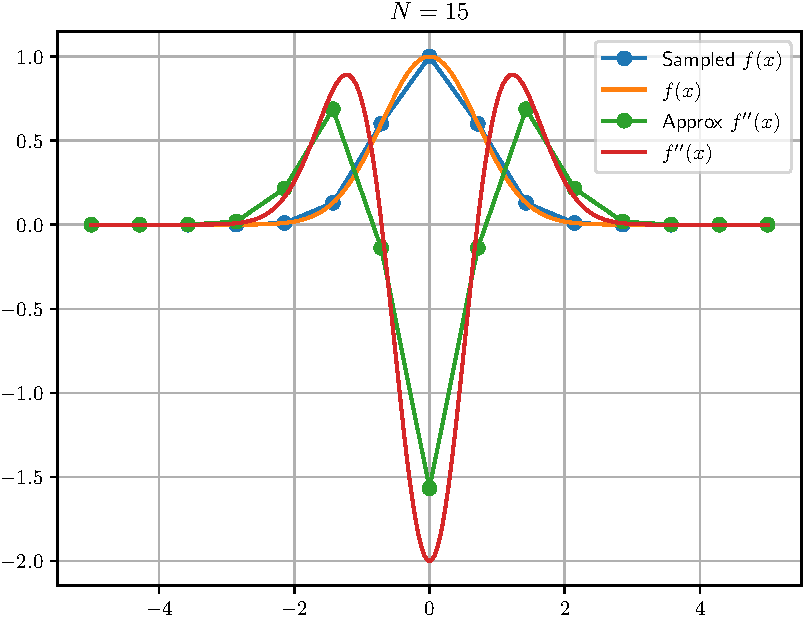
\includegraphics[scale=0.75]{codes/1d/IMG_gaussian_15.pdf}
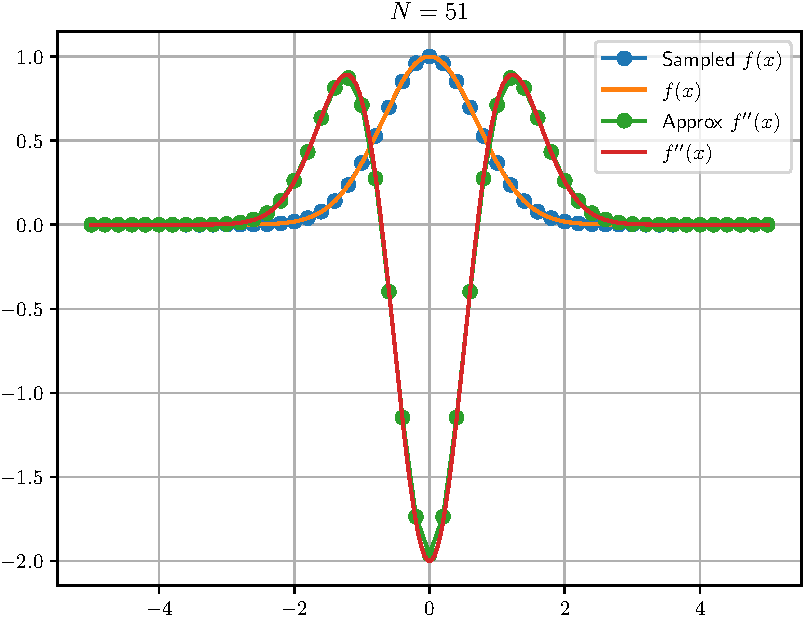
\includegraphics[scale=0.75]{codes/1d/IMG_gaussian_51.pdf}
\par}
\caption{Finite difference approximation to a Gaussian function and its second derivative}
\end{figure}


\section{Harmonic potential}

We will start with a simple potential with known exact solution, namely the harmonic potential:
\begin{equation}
V(x) = \frac{1}{2}\omega^2 x^2
\end{equation}

The Hamiltonian in finite difference representation:
\begin{equation}
\mathbb{H} = -\frac{1}{2}\mathbb{D}^{(2)} + \mathbb{V}
\end{equation}
where $\mathbb{V}$ is a diagonal matrix whose elements are:
\begin{equation}
\mathbb{V}_{ij} = V(x_{i})\delta_{ij}
\end{equation}


Code to solve harmonic oscillator:

\inputminted[breaklines,fontsize=\scriptsize]{julia}{codes/1d/main_harmonic_01.jl}

Compare with analytical solution.

Plot of eigenfunctions:

\begin{figure}[H]
{\center
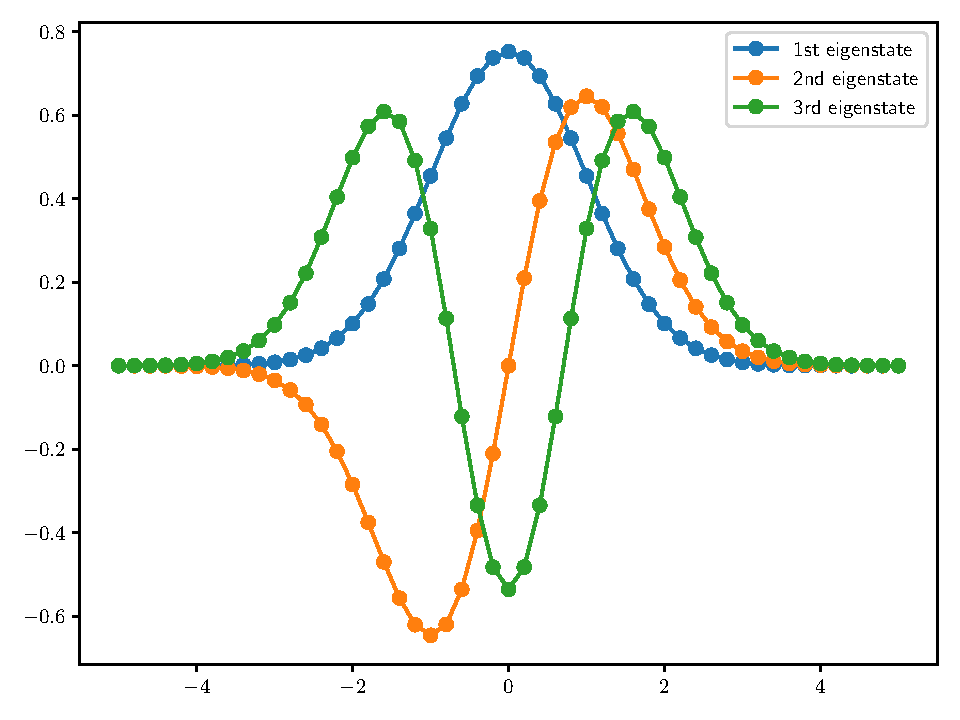
\includegraphics[scale=0.75]{codes/1d/IMG_main_harmonic_01_51.pdf}
\par}
\caption{Eigenstates of harmonic oscillator}
\end{figure}


\section{Higher order finite difference}

To obtain higher accuracy

Implementing higher order finite difference.


\section{Exercises}

Gaussian potential

